%--------------------------------------
% Create title frame
\titleframe

%--------------------------------------
% Table of contents
\begin{frame}{Overview}
  \setbeamertemplate{section in toc}[sections numbered]
  \tableofcontents[hideallsubsections]
\end{frame}


%==============================================
\section{Introduction}
%==============================================
\begin{frame}{\insertsectionhead}
  \framesubtitle{General context of the project}
\textbf{\textsc{The goal:}}\xspace Application for monitoring contracts for the delegated management of urban bus transport
\begin{figure}[ht!]
  \hspace{\fill}
  \begin{subfigure}[b]{0.3\textwidth}
    \frame{
\includegraphics[width=\textwidth]{images/mainicon.png}}
    \caption*{Application Logo}
  \end{subfigure}
  \hspace{\fill}
\end{figure}
\end{frame}

%--------------------------------------
\subsection{Host organization}
\begin{frame}
  \frametitle{\insertsectionhead}
  \framesubtitle{\insertsubsectionhead}

  \begin{columns}[T,onlytextwidth]
    \column{0.55\textwidth}
    \begin{figure}
      
\includegraphics[width=0.6\textwidth]{images/logo-uir2.jpg}
    \end{figure}
    \column{0.45\textwidth}
    What is \textbf{\textsc{UIR?}}
    \begin{description}
      \item[Creation] 2010,
      \item[Trained Executives] more than 10 000,
      \item[Partners] 30 Enterprises,
      \item[Formation Centers] 2\dots
    \end{description}
  \end{columns}
\end{frame}

%--------------------------------------

\subsection{Client and Partners}
\begin{frame}{\insertsectionhead}
  \framesubtitle{\insertsubsectionhead}
  \begin{columns}[T,onlytextwidth]
    \column{0.28\textwidth}
    Technical consulting partner
    \begin{figure}
      
\includegraphics[width=0.6\textwidth]{images/dynit.png}
    \end{figure}
    \column{0.30\textwidth}
    Client: \textbf{\textsc{DGCT}}
    \begin{figure}
      
\includegraphics[width=0.8\textwidth]{images/logo-fr.png}
    \end{figure}
    \column{0.42\textwidth}
    Its Roles
    \begin{itemize}
          \item Planning and territorial development
          \item Assistance to local public networks, and
          local institutions
          \item Improvement of urban mobility and
          transport
    \end{itemize}
  \end{columns}
\end{frame}

%--------------------------------------

\subsection{Problematic and Goals}
\begin{frame}{\insertsectionhead}
  \framesubtitle{\insertsubsectionhead}
  \textbf{\textsc{How can we improve monitoring and 
  processing of delegated transport management contracts
  urban by bus?}}
\begin{itemize}
  \item Centralize the information contained in management contracts
  delegate and their amendments, if applicable;
  \item Centralize the documents required by the contract that the operator is
  required to provide periodically to the delegating authority;
  \item Allow users to share information internally
  and documents;
  \item Monitor the management of urban transport contracts.
\end{itemize}
\end{frame}
%==============================================
\section{Project Management}
%==============================================

\subsection{Project Actors}

\begin{frame}[fragile=singleslide]{\insertsectionhead}
  \framesubtitle{\insertsubsectionhead}
  The general style for the title, section and regular frames can be changed
  easily with simple options. Here are some examples for the title page
  \begin{figure}[ht!]
    \begin{subfigure}[b]{0.3\textwidth}
      \frame{
\includegraphics[scale=0.4]{images/usertie.png}}
      \caption*{Product Owner: Mrs. Mr.Labiz Brahim}
    \end{subfigure}
    \hspace{\fill}
    \begin{subfigure}[b]{0.3\textwidth}
      \frame{
\includegraphics[scale=0.4]{images/usertie.png}}
      \caption*{SCRUM Master: Mrs.Talhaoui Insaf}
    \end{subfigure}
    \hspace{\fill}
    \begin{subfigure}[b]{0.3\textwidth}
      \frame{
\includegraphics[scale=0.4]{images/usertie.png}}
      \caption*{Developer: Mr. Kotbi Abderrahmane}
    \end{subfigure}
  \end{figure}
\end{frame}

%--------------------------------------
\subsection{Working Steps}
\begin{frame}[fragile=singleslide]{\insertsectionhead}
  \framesubtitle{\insertsubsectionhead}
  \begin{figure}[b]
    \frame{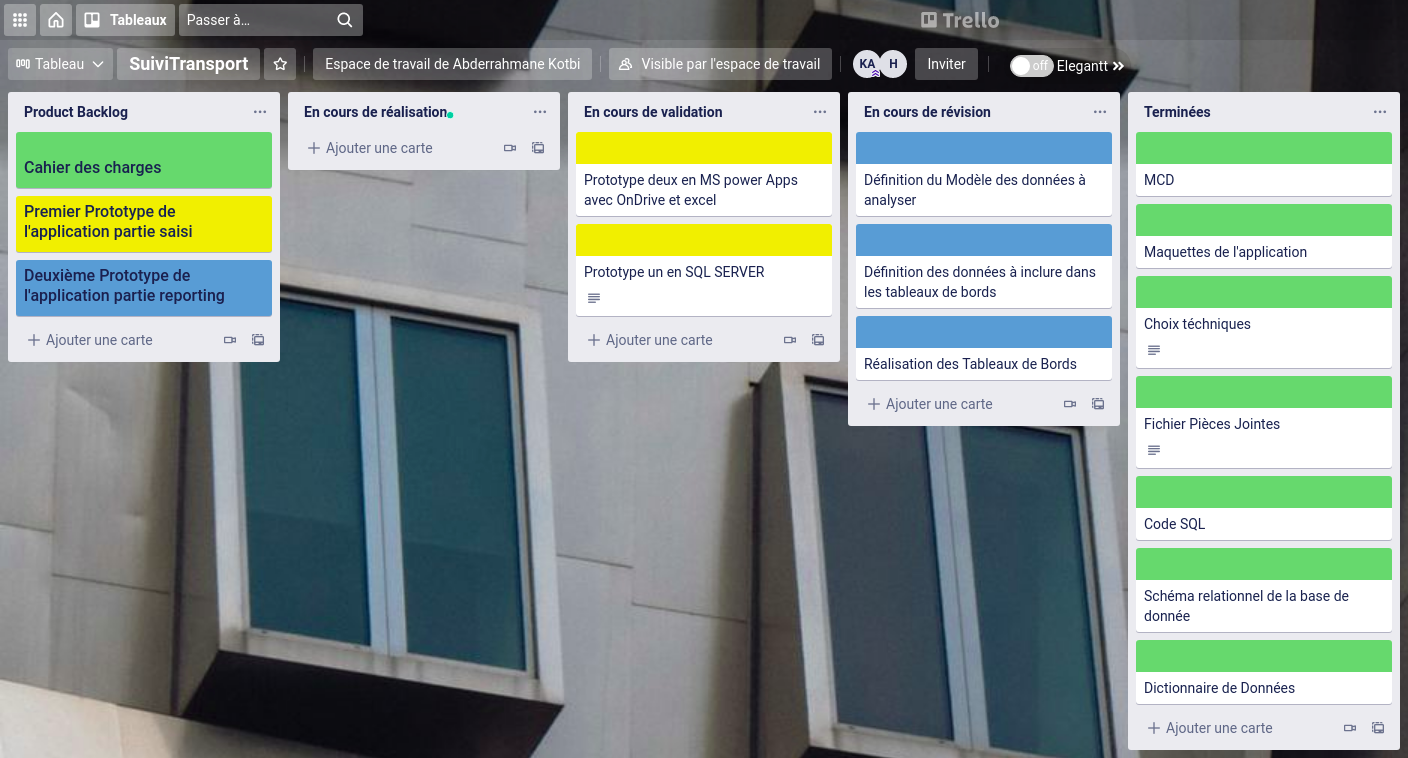
\includegraphics[scale=0.2]{images/trello.png}}
  \end{figure}
\end{frame}

%==============================================
\section{Functional Analysis and Conceptual Study}
%==============================================
\subsection{Functional Analysis}
\begin{frame}[fragile=singleslide]{\insertsectionhead}
  \framesubtitle{\insertsubsectionhead}
  \begin{figure}[b]
    \frame{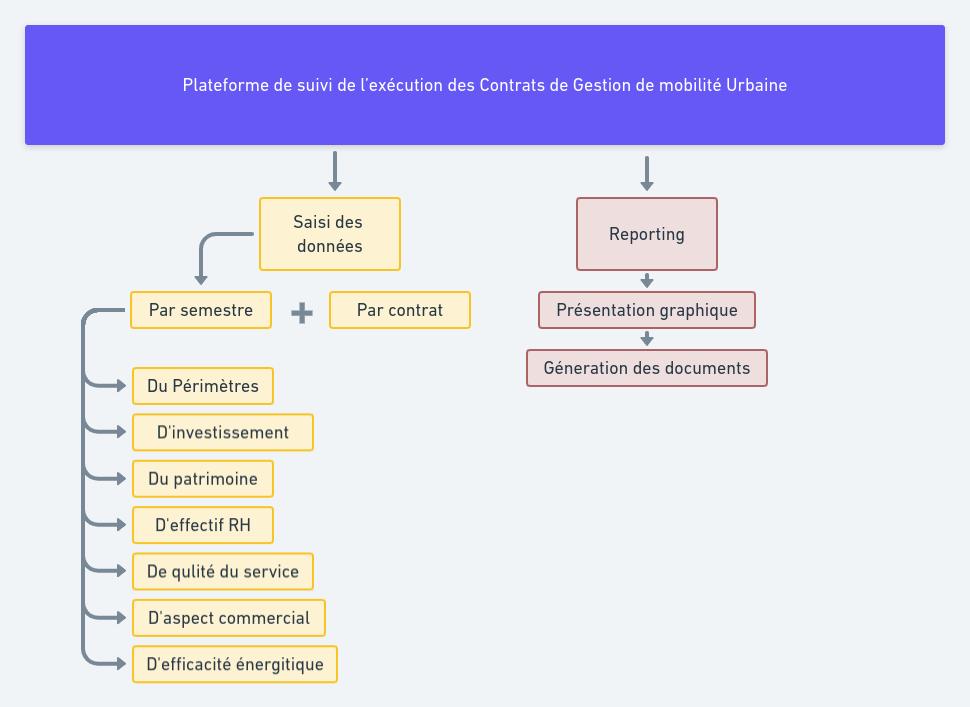
\includegraphics[scale=0.21]{images/WBS KPI.png}}
  \end{figure}
\end{frame}

%--------------------------------------

\subsection{Solution}
\begin{frame}[fragile=singleslide]{\insertsectionhead}
  \framesubtitle{\insertsubsectionhead}
  \begin{figure}[b]
    \frame{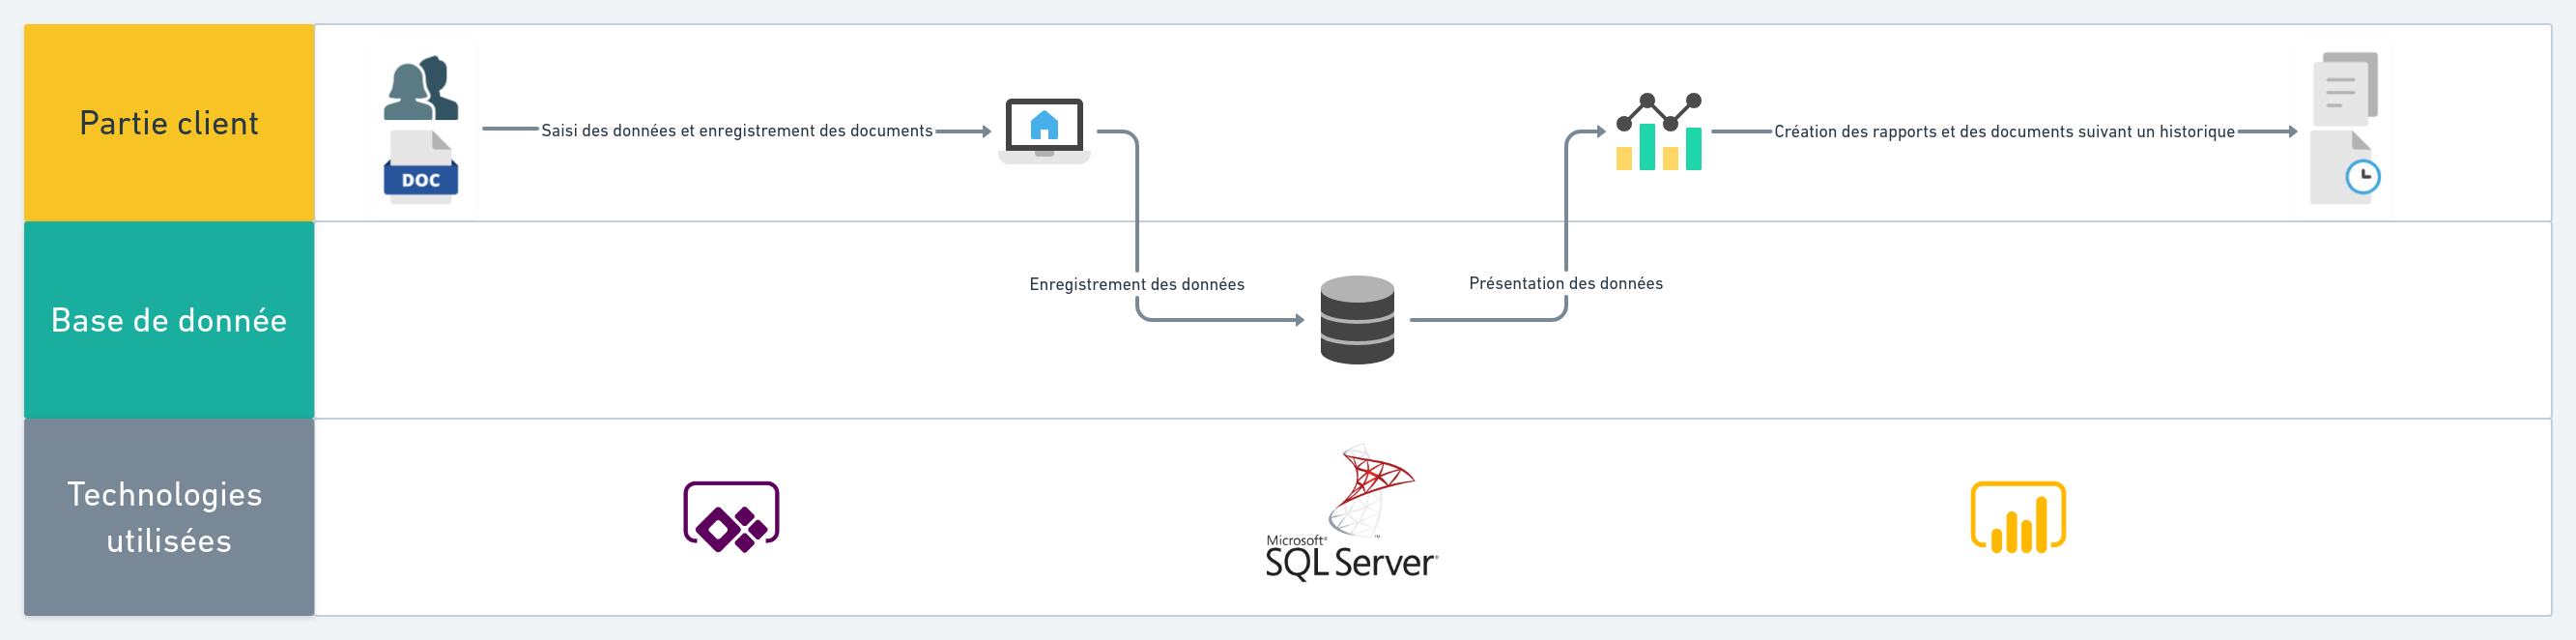
\includegraphics[width=\textwidth]{images/descrip-projet.png}}
  \end{figure}
\end{frame}

%--------------------------------------

\subsection{Conceptual study}
\begin{frame}[fragile=singleslide]{\insertsectionhead}
  \framesubtitle{\insertsubsectionhead}
  Conception
  \begin{itemize}
    \item[•] \textbf{Diagrammes réalisés:} \href{https://viewer.diagrams.net/?tags=&highlight=0000ff&edit=_blank&layers=1&nav=1&title=Diagram.drawio#Uhttps%3A%2F%2Fraw.githubusercontent.com%2Fabdorah%2Fstage2021%2Fmaster%2Fdiagramms%2FDiagram.drawio}{\textit{Page Draw.io}}
		\item[•] \textbf{Maquettes du projet:} \href{https://whimsical.com/kdi-ux-design-J9PD866564ibwyMBwLHN9N}{\textit{Page Whimsical}}
  \end{itemize}
\end{frame}

%==============================================
\section{Implementation}
%==============================================

\subsection{Welcome Page}
\begin{frame}[fragile=singleslide]{\insertsectionhead}
  \framesubtitle{\insertsubsectionhead}
  \begin{figure}[b]
    \frame{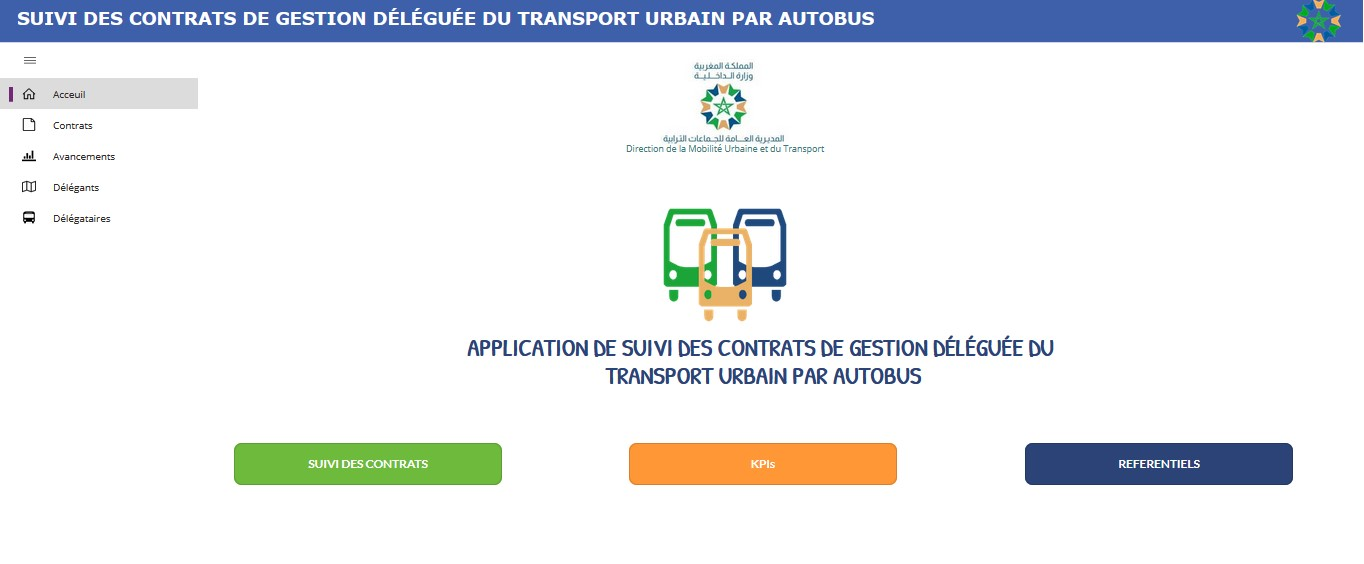
\includegraphics[width=0.9\textwidth]{images/acceuil.jpg}}
  \end{figure}
\end{frame}

%--------------------------------------

\subsection{Listing Page Example}
\begin{frame}[fragile=singleslide]{\insertsectionhead}
  \framesubtitle{\insertsubsectionhead}
  \begin{figure}[b]
    \frame{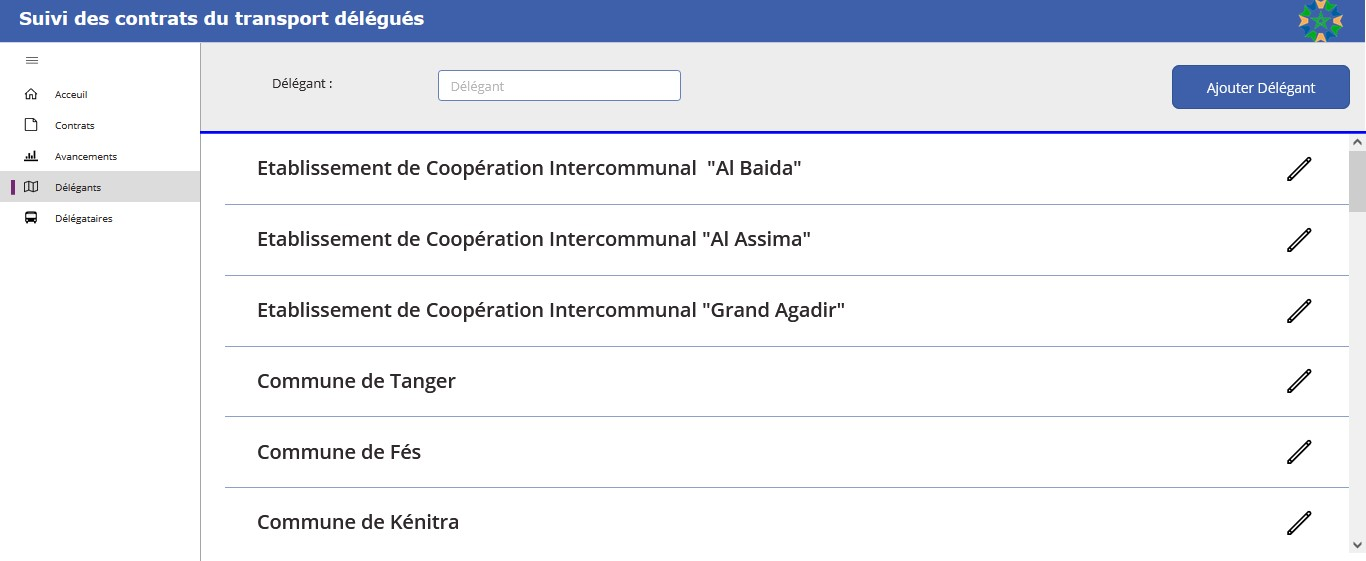
\includegraphics[width=0.9\textwidth]{images/aff delegant.jpg}}
  \end{figure}
\end{frame}

%--------------------------------------

\subsection{Display Page Example}
\begin{frame}[fragile=singleslide]{\insertsectionhead}
  \framesubtitle{\insertsubsectionhead}
  \begin{figure}[b]
    \frame{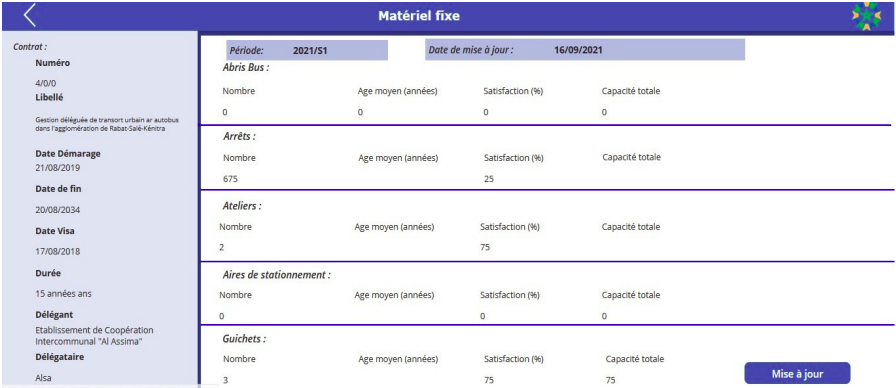
\includegraphics[width=0.8\textwidth]{images/affAv.png}}
  \end{figure}
\end{frame}

%--------------------------------------

\subsection{Add Page Example}
\begin{frame}[fragile=singleslide]{\insertsectionhead}
  \framesubtitle{\insertsubsectionhead}
  \begin{figure}[b]
    \frame{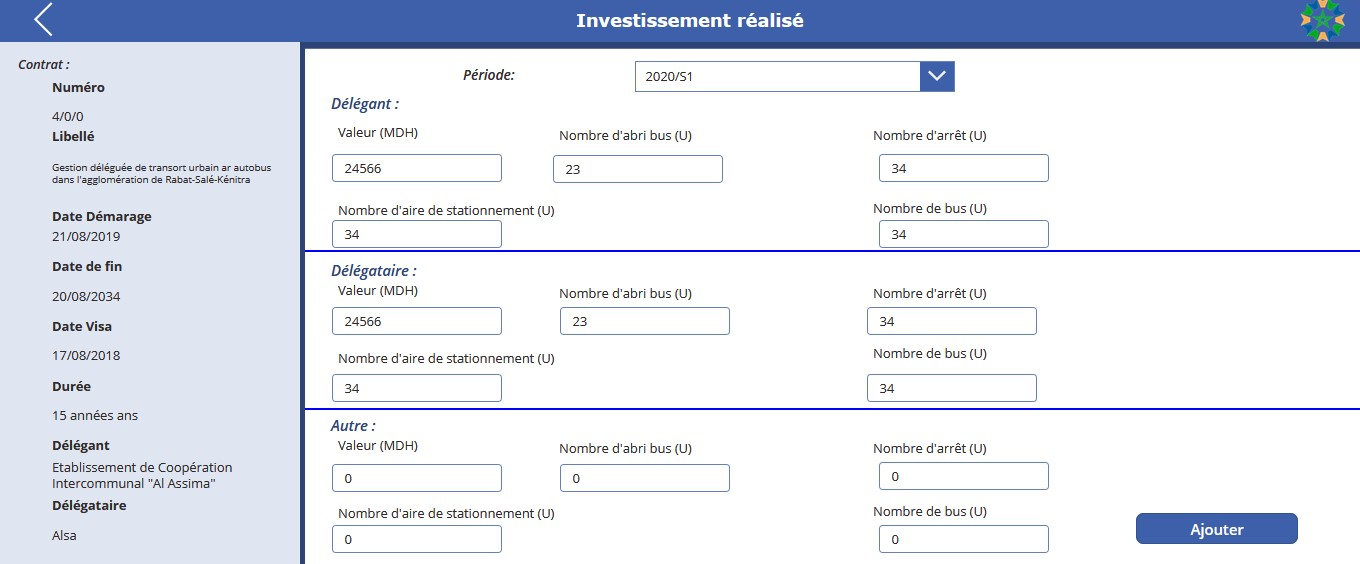
\includegraphics[width=0.9\textwidth]{images/Nv avancement invest realise.jpg}}
  \end{figure}
\end{frame}

%--------------------------------------

\subsection{Update Page Example}
\begin{frame}[fragile=singleslide]{\insertsectionhead}
  \framesubtitle{\insertsubsectionhead}
  \begin{figure}[b]
    \frame{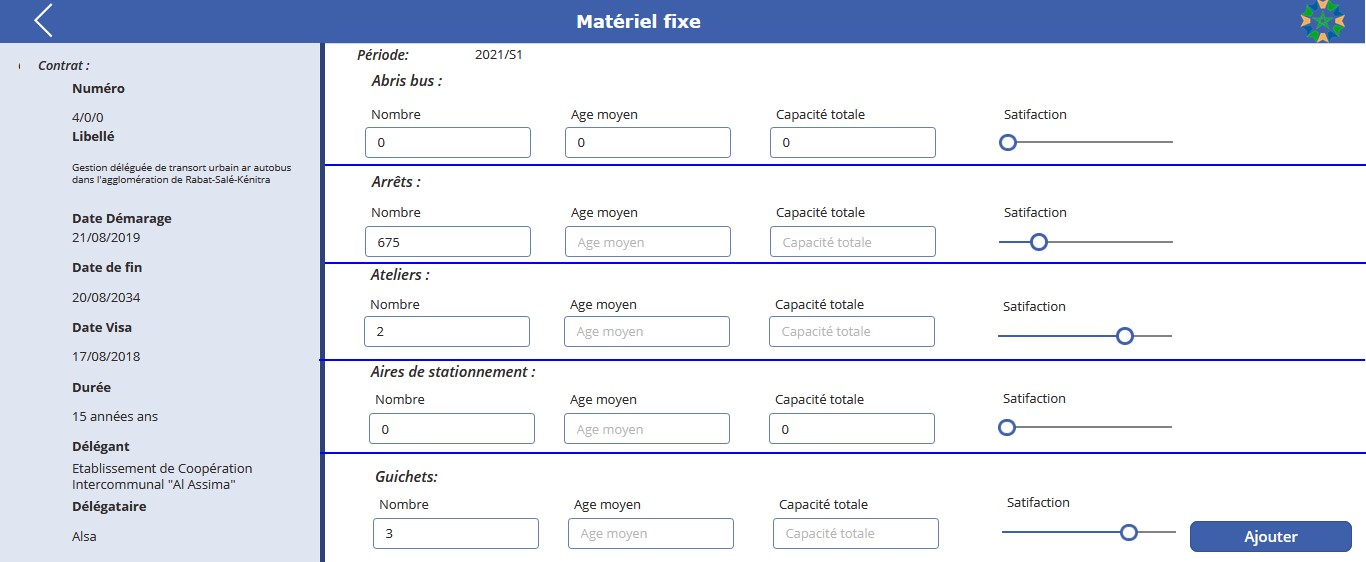
\includegraphics[width=0.9\textwidth]{images/mise a jour materiel fixe.jpg}}
  \end{figure}
\end{frame}

%==============================================
\section{Conclusion and Prescriptives}
%==============================================

\subsection{Summary}
\begin{frame}
  \frametitle{\insertsectionhead}
  \framesubtitle{\insertsubsectionhead}
  \begin{exampleblock}{Achieved}
    Data saving and presentation
  \end{exampleblock}
  \begin{alertblock}{Prescriptives}
    Reports presentation and generation in Power BI
  \end{alertblock}
  \begin{exampleblock}{Example block}
    No difference with regular block to avoid excessive distraction
  \end{exampleblock}
\end{frame}
